\section{Implementation Details}
\label{app:implementation}
\paragraph{Coordinate and object contract.}
The origin is the workspace's bottom-left corner; positions are metres and angles are radians counterclockwise from $+x$, modulo $\pi$. Image coordinates are $p_x=576x/0.6-0.5$, $p_y=384(1-y/0.4)-0.5$. Each object is encoded as
\begin{equation}
 o_i=[x_i/0.6,\ y_i/0.4,\ a_i/0.6,\ b_i/0.4,\ \cos(2\theta_i),\ \sin(2\theta_i),\ c_i^{(1:3)},\ q_i^{(1:3)}],
\end{equation}
where $a_i,b_i$ are predicted major/minor dimensions and $c_i,q_i$ are color/shape probabilities. Inference accepts one to eight detections; evaluated scenes contain two to eight objects.

\begin{table}[H]
\centering\small
\caption{Implementation dimensions and decisions in the adopted inference path.}
\begin{tabularx}{\linewidth}{@{}lY@{}}\toprule
\textbf{Component} & \textbf{Implementation} \\\midrule
Perception & RT-DETR-R18; 3 decoder layers; 300 width-256 queries; internal $640\times640$ input. \\
Appearance adapter & $16\times16$ predicted-box crop; CNN $3\to16\to32$; query/crop head $288\to128\to10$. \\
Size residual & $8\times8$ crop; 16-channel CNN feature + query; MLP $272\to64\to2$; dimension floor $10^{-4}$\,m. \\
Language & MiniLM tokens $384\to128$; 7 goal queries; four-head text attention; feed-forward $128\to512\to128$. \\
Goal / selection & Text-only goal: keep (1), axis (2), region (3), gap (3), grouping (2), order (2). Separate selection: object $12\to128$, self-/language attention, head $128\to1$. \\
Relation / context & MLP $12\to128\to128$; one width-128, four-head set-attention block for structure. \\
Structure & Row MLP $141\to128\to8$; pointer query $269\to128\to128$, masked dot-product selection. \\
Pose heads & Row origin $417\to128\to2$; X step $3\to32\to1$; angle $141\to128\to2$, half-atan2 decoding. \\
Filtering / search & Foreground threshold 0.5; duplicate-center radius 10\,mm; at most eight checked candidates per search. \\\bottomrule
\end{tabularx}
\end{table}

For keep probability $k$ and attribute distributions $p_a,p_r,p_\delta,p_c,p_s$, the goal is $g=[k,(1-k)p_a,(1-k)p_r,(1-k)p_\delta,(1-k)p_c,(1-k)p_s]$. Tokens $z_i=h_i+W_g g+W_s s_i$ are normalized before self-attention is added to $h_i$; a null key handles padding. Context guides row/order selection; pose heads use original $h_i$. Rows and pointer prefixes are predicted at inference, with teacher forcing only in training. Each row shares its neural origin's $y$ coordinate; positive X steps use $\operatorname{softplus}(\operatorname{MLP}([w_{j-1},w_j,\delta]))$.

The ideal axis-aligned spacing is
\begin{equation}
 x_{j+1}-x_j=\tfrac12(w_j+w_{j+1})+\delta,\qquad
 y_r-y_{r+1}=\tfrac12(H_r+H_{r+1})+\delta_r,
\label{eq:spacing}
\end{equation}
where $w_j$ is horizontal extent, $H_r$ the maximum row height, and $\delta_r=2\delta$ between color bands ($\delta$ otherwise). The implemented decoder uses rotated rectangles and $\pm2$\,mm gap bands rather than exact equalities. Regions $(x_{\min},y_{\min},x_{\max},y_{\max})$ are full $(.02,.02,.58,.38)$, left $(.02,.02,.28,.38)$, and right $(.32,.02,.58,.38)$; a fitting layout may shift 1\,mm inward.

The initial search ranks candidates by row and pointer scores; repair/color-split searches use row scores. Enumeration may consider more partitions before truncation. Explicit area-order enforcement applies on the full route and in invoked repair, not universally on the partial route. Exhausted repair retains the original prediction: neither feasibility nor global optimality is guaranteed. Preservation details appear in Appendix~\ref{app:qualitative}.

\clearpage
\section{Training Evidence and Optimization}
\label{app:training}
\begin{table}[H]
\centering\small
\caption{Recorded training stages. These are stage-specific exposures, not repeated full-corpus training. The official test and independent final holdout are excluded.}
\begin{tabularx}{\linewidth}{@{}lY@{}}\toprule
\textbf{Stage} & \textbf{Evidence and scope} \\\midrule
Base integration & Separate perception and arrangement checkpoints at updates 2,400 and 6,000, respectively. \\
Relation stages & 791 training and 94 validation pairs; seed 1203. The final pipeline reuses only the relation hidden encoder. \\
Size residual & 3,200 train source families, divided into 2,560 fit / 640 development; batch 8; learning rate $10^{-3}$; selected update 200. \\
Restricted joint & Official train families split 4/5 fit, 1/5 development; batch 4; AdamW, learning rate $10^{-5}$, weight decay 0; 30 updates, 120 attempted presentations, 6 excluded. \\
Set selector & 1,792 eligible train families, 5,376 full pairs, 5,085 usable; 249 association and 42 count exclusions; 8 epochs / 1,272 updates; initial learning rate $10^{-4}$; selected epoch 1. \\
Broad joint pilot & Seed 1203; batch 2; encoder / goal / hidden / row learning rates $10^{-6}/10^{-5}/10^{-5}/10^{-4}$; stopped at update 200 after collapse; not adopted. \\\bottomrule
\end{tabularx}
\end{table}

\paragraph{Losses and gradient boundaries.}
Write the SmoothL1 penalty as $H_\beta(e)=e^2/(2\beta)$ if $|e|<\beta$, and $|e|-\beta/2$ otherwise. Let $d_\pi(\alpha,\beta)=((\alpha-\beta+\pi/2)\bmod\pi)-\pi/2$. The size residual minimizes
\begin{equation}
 \mathcal L_{\mathrm{size}}=\operatorname{mean}_{i\in M,k\in\{a,b\}}H_{.001}(\hat s_{ik}-s^*_{ik}).
\end{equation}
$M$ denotes matched objects. Matching uses true source centers only during supervision; detector outputs and predicted crop boxes are detached. The selector's recorded objective is row cross-entropy plus teacher-forced pointer cross-entropy,
\begin{equation}
 \mathcal L_{\mathrm{select}}=\operatorname{CE}(R,r^*)+\operatorname{CE}(O,\pi^*),
\end{equation}
with invalid/padded targets ignored. The recorded total equals these two losses; no extra color regularizer is assumed.

In restricted joint fine-tuning, let $G$ contain reference predictions within 2\,mm position error and $3^\circ$ angle error, and $F$ contain the other valid objects. The recorded objective is
\begin{align}
\mathcal L_{\mathrm{joint}}={}&\mathcal L_{\mathrm{size}}
+\operatorname{mean}_{i\in F,k\in\{x,y\}}H_{.010}(\hat p_{ik}-p^*_{ik})
+\operatorname{mean}_{i\in F}|d_\pi(\hat\theta_i,\theta_i^*)|\nonumber\\
&+\operatorname{mean}_{i\in G,k\in\{x,y\}}H_{.001}(\hat p_{ik}-p^{\mathrm{ref}}_{ik}).
\end{align}
Empty terms are zero. Only the size residual, horizontal step head, and final row-origin layer update. Refined sizes are stop-gradient before the pose forward pass; perception, language, goal, relation, structure, and angle heads are frozen. Consequently the angular term contributes to the loss value but cannot update the frozen angle head. This is a restricted multi-head update, not a differentiable joint objective through the entire system.

\paragraph{Development evidence and its limits.}
The saved 152-scene full-arrangement diagnostic improves from 24 to 42 successes after size refinement and from 42 to 54 after restricted joint tuning. Size refinement reduces median major-dimension error from 1.419 to 0.790\,mm (796 matched objects), while restricted joint tuning reduces median vertical-gap error from 2.015 to 1.588\,mm. These are recorded development stages with evolving code and selection gates, not independent final-test ablations. In contrast, the broader joint pilot falls from 2/38 to 0/38 development successes and from 24/152 to 1/152 validation successes at update 200; the best checkpoint remains update 0. A historical 260-scene diagnostic overlapped earlier fitting data and is excluded from claims of independent generalization.

\clearpage
\subsection{Selector Learning Curve}
\begin{figure}[H]
\centering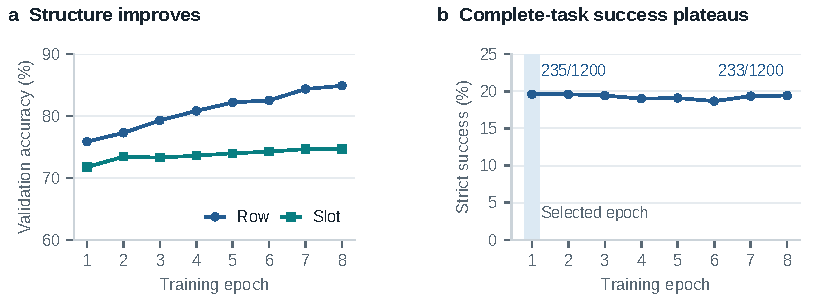
\includegraphics[width=\linewidth]{figures/selector_training.pdf}
\caption{Historical selector-stage validation on 1,200 full-arrangement pairs, before the final inference refinements. Row and slot accuracy improve, but complete-scene success plateaus. This is a component-training diagnostic, not the final independent evaluation. Values are read from the saved eight-epoch curve.}
\label{fig:training}
\end{figure}

The baseline succeeds on 222/1200 pairs. Epoch 1 reaches 235/1200, with row/slot accuracy of 75.86\%/71.77\% (baseline: 68.52\%/61.87\%). Mixed-color-row tags fall from 234 to 22. At epoch 8, row/slot accuracy reaches 84.88\%/74.68\%, but success is 233/1200. Improved structure need not remove a scene's last violation.

\section{Data and Statistical Details}
\label{app:statistics}
Scene and asset seeds are 120912 and 120913, respectively. Major dimensions span 40--80\,mm, minor dimensions 25--50\,mm, and heights 5--20\,mm on a 1\,mm grid, with aspect ratio $\geq1.3$. The corpus uses \code{continuous\_rows\_v3} teacher layouts and \code{english\_rows\_v1} instructions. For family $i$, bucket $\lfloor i/20\rfloor\bmod10$ assigns 0--7 to train, 8 to validation, and 9 to test. These pools also use mutually disjoint sets of 64 asset families each. Source clearance/margin is 12\,mm; accepted targets require 10\,mm and exact source copies for locked poses. Independent validation checks targets. Dataset RGB rendering used Blender 5.1.0, Cycles CPU, and 32 samples; PNG bytes may vary across environments.

The separate final set uses scene seed 20261112, registry seed 120913, and development assets. Its 128 families/640 pairs share no geometry-family IDs, RGB hashes, or asset-family IDs with the corpus. This tests new instances within the procedural domain. Mode labels follow teacher outcomes: already-satisfied color-selective commands become no-op. Actual mode counts determine denominators.

\paragraph{Paired bootstrap.}
Define $d_f=\frac15\sum_{j=1}^{5}(Y^{v2}_{fj}-Y^{v1}_{fj})$. Resample 128 families with replacement and compute $100\operatorname{mean}_f d_f$, preserving five paired outcomes per family. Python's local random generator (seed 20261112) produces 10,000 replicates; sorted indices 250 and 9749 give 4.84375 and 11.5625 points. The observed gain is 7.96875 points. Paired counts are 489 both-pass, 51 v2-only, 0 v1-only, and 100 both-fail. This reaggregation does not rerun model evaluation.

\begin{table}[H]
\centering\small
\caption{All nonzero error tags across either release. Tags overlap; horizontal and vertical gaps coincide in 20 v2 scenes.}
\begin{tabular*}{\linewidth}{@{}l@{\extracolsep{\fill}}rrlrr@{}}\toprule
\textbf{Error} & \textbf{v1} & \textbf{v2} & \textbf{Error} & \textbf{v1} & \textbf{v2} \\\midrule
Horizontal gap & 51 & 49 & Clearance & 9 & 7 \\
Vertical gap & 48 & 42 & Keep pose & 9 & 4 \\
Object count & 45 & 5 & Mixed-color row & 2 & 0 \\
Requested region & 17 & 4 & Collision & 1 & 0 \\
Size order & 13 & 11 & Boundary & 1 & 0 \\\bottomrule
\end{tabular*}
\end{table}

\clearpage
\section{Command Dependence and Object Correspondence}
\label{app:qualitative}
\begin{figure}[H]
\centering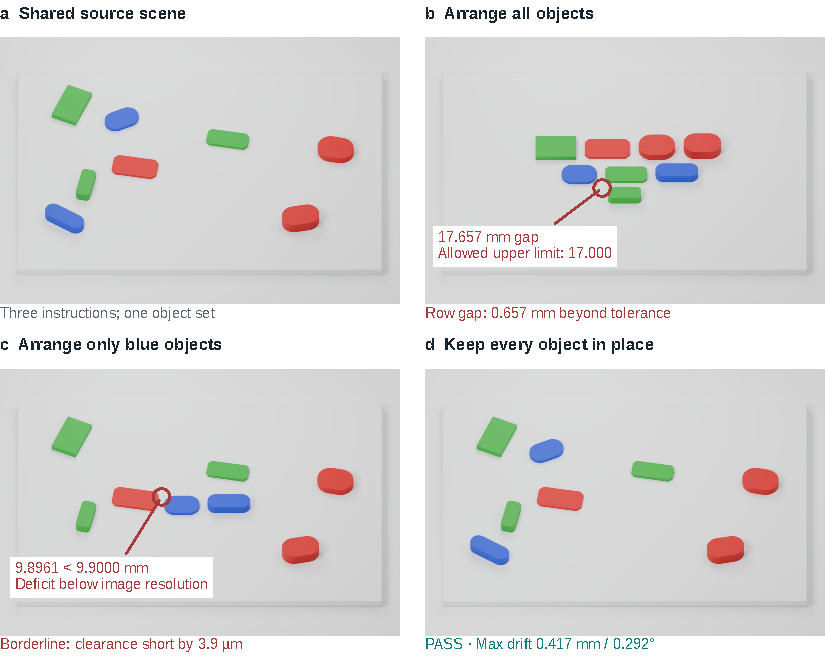
\includegraphics[width=\linewidth]{figures/qualitative_modes.pdf}
\caption{One validation scene under three commands, rendered with the same Blender camera and lighting. (b) fails because a row gap is 0.657\,mm past its upper limit. (c) fails clearance by 3.9\,$\mu$m, a deficit this print cannot resolve. (d) passes, with at most 0.42\,mm and 0.29$^\circ$ of drift from the source. Figure~\ref{fig:diagnostics} measures (b) and (c) on overhead crops.}
\label{fig:modes}
\end{figure}

\paragraph{Preservation implementation.}
For an unambiguous named color, partial mode replaces the moving set with those objects. Held objects constrain a static clearance search that translates the moving block on a 5\,mm grid within $\pm120$\,mm. Held/no-op angles use silhouette PCA on connected components in a local $\pm80$\,mm image window, with chroma threshold $25/255$ and at least 40 pixels. If PCA is unavailable, a direction head supplies the angle; without its checkpoint, the base detector angle is retained. This is static placement, not grasp or trajectory planning.

\paragraph{Pose-change notation.}
Figure~\ref{fig:motion} measures $d_i=1000\|\hat p_i-p_i^{\mathrm{src}}\|_2$ in millimeters and
\begin{equation}
\Delta\theta_i=\frac{180}{\pi}\left[\left(\hat\theta_i-\theta_i^{\mathrm{src}}+\frac\pi2\right)\bmod\pi-\frac\pi2\right].
\end{equation}
IDs match the saved scene objects. Source poses are original scene-record poses, and targets are stored model predictions. World-plane vectors and orientation glyphs describe pose differences only; they do not imply a collision-free manipulation path or an executed robot motion.

\paragraph{Example provenance.}
The smoke script chose the first supported example of each mode from family \code{expanded\_09aa3f57968449ce8a09f291}, with suffixes \code{\_0}, \code{\_2}, and \code{\_3}. The full and partial commands request horizontal axes and 15\,mm gaps; partial selects blue objects. No-op maximum drift is 0.417\,mm and $0.292^\circ$. The six-object opening example is \code{expanded\_e2ee7a75ae3a34826b36d71f\_0}; the eight-object motion example is \code{expanded\_717287879ce16878c5558650\_4}. These selected validation records lack per-record checkpoint digests and illustrate behavior, not a second benchmark. The older ten-image v1 gallery is not used as v2 evidence.

\clearpage
\section{Failure Margins and Rendering Fidelity}
\label{app:failure}
\begin{figure}[H]
\centering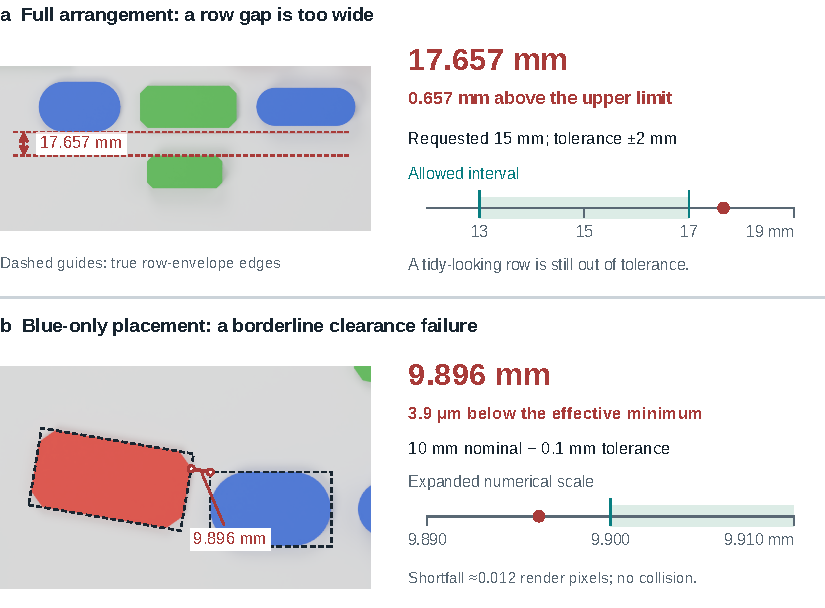
\includegraphics[width=\linewidth]{figures/failure_explanation.pdf}
\caption{Measured violations, not just failure labels. Real Blender closeups mark the evaluated bounding envelopes; the adjacent rulers compare each measured value with its permitted interval. The row gap exceeds 17.000\,mm by 0.657\,mm. Clearance falls about 3.9\,$\mu$m below 9.900\,mm, after the evaluator's 0.1\,mm numerical tolerance. Ruler scales differ and are labeled explicitly.}
\label{fig:diagnostics}
\end{figure}

\paragraph{Why the borderline example matters.}
The partial result is not evidence of a visually poor arrangement or a physical collision. Its failure is a precise consequence of the synthetic evaluator's envelope-distance threshold. True mesh silhouettes and oriented bounding rectangles differ, especially for capsules and chamfers; the annotated quantity is rectangle-to-rectangle clearance. This example motivates distinguishing failure severity and scoring margins from a binary success rate. It supplies no estimate of how frequently such near-threshold cases occur across the holdout.

\paragraph{Pose and geometry fidelity.}
Every presentation image renders a preserved scene record. Meshes extrude the project's original footprint polygons to their recorded heights, retaining identity, color, dimensions and source/predicted pose. No layout is adjusted for composition. Before/after views share orthographic camera, illumination, materials, background, and image quality. Blender 5.1.0 uses Cycles CPU, $1920\times1280$ resolution, denoising and adaptive sampling with a 128-sample maximum. Overhead closeups use the same materials and lighting with a calibrated camera.

The original $576\times384$ RGB images remain the actual inference inputs (one appears in Figure~\ref{fig:architecture}); presentation renders are generated only afterward. Input/output hashes, object transforms, camera settings, editable Blender scenes and scripts are included. An independent check reopens every saved scene and compares all object transforms and mesh vertices with the source records. The only residual differences are float32 storage quantization, below $10^{-7}$ in the corresponding meter/radian coordinates. No additional model inference or training is performed.

\clearpage
\section{Reproducibility and Evidence Package}
\label{app:reproducibility}
The analysis compares v1.0.0 (\code{26dca53}) and v2.0.0 (\code{593bd5d}); the release-candidate measurement was carried forward without changing inference. Manuscript preparation used checkout \code{535f14f}. The adopted entry points are \code{load\_adopted} in the end-to-end scorer and \code{poses\_from\_detection} in \code{size\_refinement.py}. Source-identity matching minimizes a Hungarian cost incorporating confidence, source position, size, and angle. Each match must additionally satisfy center distance $\leq10$\,mm and oriented-envelope IoU $\geq0.5$; otherwise the scene fails with \code{source\_identity}. Target poses then undergo the independent semantic and geometry checks.

The model runtime uses Python 3.12, PyTorch 2.9.1, torchvision 0.24.1, and transformers 4.57.3. The text backbone is \code{paraphrase-multilingual-MiniLM-L12-v2}; pretrained snapshots are pinned in \code{configs/pretrained\_rtdetr.json}. Reloading requires local base/parent checkpoints, relation, joint row/size and selector weights, selection/direction heads, and pretrained caches. The source repository does not distribute these weights or datasets, and the historical selector trainer and independent-set generator are absent. The package below supports reproduction of the \emph{paper's analysis and figures}, rather than claiming full training reproduction.

\paragraph{Version-controlled change.}
The v1.0.0--v2.0.0 changes are inference refinements: duplicate suppression, sentence-consistent region/gap choices, exact named-color mover replacement, infeasible-row repair, and feasible color-row splitting. Architecture, loading paths, set attention, size residual, constraint search, and PCA correction are shared. Individual effects remain unmeasured.

\begin{table}[H]
\centering\small
\caption{Manuscript evidence package. Paths are relative to the submission root. Full SHA-256 values and original paths are preserved in the audit manifests.}
\label{tab:package}
\begin{tabularx}{\linewidth}{@{}lY@{}}\toprule
\textbf{Artifact} & \textbf{Purpose} \\\midrule
\code{audit/evidence/v1\_holdout.jsonl} & Frozen baseline scores; SHA-256 prefix \code{89b3ee1cbc24}. \\
\code{audit/evidence/v2\_holdout.jsonl} & Frozen v2 scores; prefix \code{209df3c1b12c}. \\
\code{audit/verified\_results.json} & Recomputed counts, breakdowns, paired gain and family bootstrap. \\
\code{scripts/audit\_results.py} & Statistical reaggregation without model inference. \\
\code{scripts/make\_figures.py} & Figure rebuild entry point; calls the publication compositor. \\
\code{scripts/render\_publication.py} & Blender source for matched views at saved poses. \\
\code{renders/} & High-resolution PNGs, editable Blender scenes, and pose/camera metadata. \\
\code{audit/evidence/} & Training summaries, qualitative poses, RGB and rendered prediction. \\
\code{audit/method\_audit.md} & Claim-to-code references and gradient boundaries. \\
\code{audit/results\_audit.md} & Claim-to-record references and dataset integrity. \\
\code{template/upstream.json} & Official ICLR template source and exact hashes. \\\bottomrule
\end{tabularx}
\end{table}

\paragraph{Compute scope.}
The selector stage records 1,719 GPU-seconds, not the total project compute. Saved timing gives median 131.5/137.2\,ms and mean 169.2/197.5\,ms for v1/v2. Hardware, warmup, and serving conditions are not controlled sufficiently for a throughput claim. No total training budget, deployment cost, or physical cycle time is established.

\paragraph{Rebuilding.}
The README provides commands and dependency pins. The analysis scripts in Table~\ref{tab:package} reconstruct the statistics and seven figures. Running \code{latexmk -pdf main.tex} compiles the manuscript. All figure PDFs are included, so compilation alone requires neither Python nor a GPU, checkpoints, or the original datasets.

\paragraph{Assistance disclosure.}
Codex assisted with repository and record inspection, primary-source literature discovery, drafting, figure scripting, and LaTeX typesetting. Experimental outcomes come from saved project records. Manuscript preparation performed statistical reaggregation and Blender visualization at fixed saved poses, without generating additional model predictions or training results.
